\section{preliminaries}

In this paper, we focus on a large unweighted and undirected bipartite graph $G = (U, V, E)$, where $U$ and $V$ are sets of vertices, and $E$ is the set of undirected edges. For each vertex $u \in U$ (or $V$), its neighbors are denoted by $N(u) = \{v \mid e(u,v) \in E\}$. The common neighbors of a vertex set $S$ are denoted as $N(S) = \bigcap_{u \in S} N(u)$. Let $d(u)$ be the degree of a vertex $u$, i.e., $d(u) = |N(u)|$.

For simplicity, we assume without loss of generality that the vertices on each side of the bipartite graph $G'$ are arranged in a particular order. Specifically, we order the vertices as $u_1 \prec u_2 \prec \dots \prec u_{n_1}$ for $U$ and $v_1 \prec v_2 \prec \dots \prec v_{n_2}$ for $V$. Additionally, we assume that $p \leq q$, with $p$ representing the number of vertices from the $U$ side and $q$ from the $V$ side. The same methods can be applied when $p > q$.

Please note that, for convenience, the examples provided in this paper consider \red{the natural ordering} of the vertices.

\begin{definition}[Biclique]
A biclique $g=(U',V',E')$ in the bipartite graph $G = (U, V, E)$ is a pair of vertex subsets $U' \subseteq U$ and $V' \subseteq V$ such that every vertex $u \in U'$ is adjacent to every vertex $v \in V'$. \ie,
$E' = \{ (u, v) \mid u \in U', v \in V' \} \subseteq E$.

\end{definition}

A biclique $B$ is called a $(p,q)$-biclique if $|U'|=p$ and $|V'|=q$.

\stitle{Problem Statement} given a large bipartite graph $G$, and two integers $p,q$, and error parameter $\epsilon \in (0,1)$ and $\delta \in (0,1)$,we study the problem of approximately counting the number of \bicliques in $G$. \ie  our main goal is to design a randomized algorithm that outputs an estimated value $\estcnt$ satisfying,

\[
P \left(\Big|\widehat{\text{cnt}}_{(p,q)}(G) - \text{cnt}_{(p,q)}(G)\Big| > \epsilon \cdot \text{cnt}_{(p,q)}(G)\right) \leq \delta
\]



\begin{center}
\begin{figure}

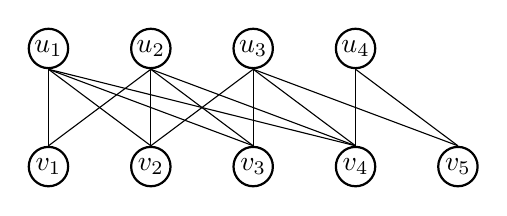
\begin{tikzpicture}[scale=1, 
	every node/.style={circle, draw, minimum size=0.5cm, inner sep=0pt, line width=0.8pt}
]
	
	% Nodes
	\node (u1) at (0,1.5) {$u_1$};
	\node (u2) at (1.3,1.5) {$u_2$};
	\node (u3) at (2.6,1.5) {$u_3$};
	\node (u4) at (3.9,1.5) {$u_4$};

	
	\node (v1) at (0,0) {$v_1$};
	\node (v2) at (1.3,0) {$v_2$};
	\node (v3) at (2.6,0) {$v_3$};
	\node (v4) at (3.9,0) {$v_4$};
	\node (v5) at (5.2,0) {$v_5$};
	
	% Edges
	\draw (u1.south) -- (v1.north);
	\draw (u1.south) -- (v2.north);
	\draw (u1.south) -- (v3.north);
	\draw (u1.south) -- (v4.north);
	\draw (u2.south) -- (v1.north);
	\draw (u2.south) -- (v2.north);
	\draw (u2.south) -- (v3.north);
		\draw (u2.south) -- (v4.north);
	
	\draw (u3.south) -- (v2.north);
	\draw (u3.south) -- (v3.north);
	
	\draw (u3.south) -- (v4.north);
		\draw (u3.south) -- (v5.north);
	

	\draw (u4.south) -- (v4.north);
	\draw (u4.south) -- (v5.north);

\end{tikzpicture}
\caption{An example graph}
\label{fig:ex1} 
\end{figure}
\end{center}
\red{change () to \{\}}\\

Consider the graph shown in Figure \ref{fig:ex1}, there are five (2,3)-bicliques
 $ \mathcal{B}_{(2,3)} = \{\{(u_1, u_2), (v_1, v_2, v_3)\}, \{(u_1, u_2), (v_1, v_2, v_4)\},\{(u_1, u_2), (v_1,\\ v_3, v_4)\},\{(u_1, u_2), (v_2, v_3, v_4)\}\},\{(u_2, u_3), (v_2, v_3, v_4)\}\} $.

%\begin{table}[htb]
%	\small
%	\caption{Frequently Used Notation}
%	\label{tab:notation}
%	\begin{tabular}{c|l} \hline
%		\textbf{Notation} & \textbf{Description} \\ \hline
%		$\mathcal{B}_{(p,q)}$ & Set of all $(p,q)$-bicliques in $G$ \\
%		$\cnt$ & Total number of $(p,q)$-bicliques in $G$, i.e., $\cnt = |\mathcal{B}_{(p,q)}|$ \\
%		$\estcnt$ & Estimated total number of $(p,q)$-bicliques in $G$ \\
%		$\Delta$ & Set of all $(p,q)$-zstars in $G$ \\
%		$\mathcal{\hat{B}}(G)$ & Biclique density of $G$, defined as $\mathcal{\hat{B}}(G) = \frac{\cnt}{|\Delta|}$ \\
%		$Z^*$ & A $(p,q)$-zstar in $G$ \\
%		$\sampelspace$ & Sample space used for estimating $\cnt$ \\
%
%		$\mathbb{S}_{(p,q)}(G)$ & The BC-Shadow sample space for $(p,q)$-bicliques in $G$ \\
%		$\mu_{\sampelspace}$ & Biclique density of the sample space $\sampelspace$, i.e., $\mu_{\sampelspace} = \frac{\cnt}{|\sampelspace|}$ \\
%		$\mathcal{P}_{(p,q)}(S_U, S_V)$ & Set of all pairs $(U', V')$ with $U' \subseteq S_U$, $V' \subseteq S_V$, $|U'|=p$, $|V'|=q$ \\
%		$N(u)$ & Neighbors of vertex $u$, i.e., $N(u) = \{ v \mid (u, v) \in E \}$ \\
%		$N(S)$ & Common neighbors of a vertex set $S$, i.e., $N(S) = \bigcap_{u \in S} N(u)$ \\
%		$d(u)$ & Degree of vertex $u$, i.e., $d(u) = |N(u)|$ \\
%		$\epsilon, \delta$ & Error parameters for approximation, with $\epsilon \in (0,1)$ and $\delta \in (0,1)$ \\
%		$\gamma$ & Parameter used in sampling algorithms, related to $\epsilon$ and $\delta$ \\
%		\hline
%	\end{tabular}
%\end{table}

\begin{table}[htb]
	\small
	\caption{Frequently used notations}
	\label{table:notations}

	\begin{tabular}{c|l} \hline
		Notation & Meaning \\ \hline
	$\setbiclique$ & Set of all $(p,q)$-bicliques in $G$ \\
	$\cnt$ & Total number of $(p,q)$-bicliques in $G$, i.e., $|\mathcal{B}_{(p,q)}|$ \\
	$\estcnt$ & Estimated total number of $(p,q)$-bicliques in $G$ \\
	$\Delta(G)$ & Set of all $(p,q)$-zstars in $G$ \\
	$\sampelspace$ & sampling space of $\setbiclique$ satisfying $\sampelspace \supseteq \setbiclique$ \\
	\shadow & BC-Shadow \\

	\end{tabular}
\end{table}


